\documentclass[12pt]{third-rep}

\usepackage{url} % typeset URL's sensibly

\usepackage{pslatex} % Use Postscript fonts

\title{CAB402 Programming Paradigms \\ \vspace{2 mm} {Quantum Computing}}
\author{Thanat Chokwijitkul n9234900}
\date{}

\usepackage{pslatex} % sets up the use of PostScript fonts

\renewcommand{\bibname}{References} % changes to references

\usepackage{listings}

\usepackage{titlesec}
\titleformat{\chapter}{\normalfont\huge\bf}{\thechapter.}{20pt}{\huge\bf}

%    Q-circuit version 2
%    Copyright (C) 2004  Steve Flammia & Bryan Eastin
%    Last modified on: 9/16/2011
%
%    This program is free software; you can redistribute it and/or modify
%    it under the terms of the GNU General Public License as published by
%    the Free Software Foundation; either version 2 of the License, or
%    (at your option) any later version.
%
%    This program is distributed in the hope that it will be useful,
%    but WITHOUT ANY WARRANTY; without even the implied warranty of
%    MERCHANTABILITY or FITNESS FOR A PARTICULAR PURPOSE.  See the
%    GNU General Public License for more details.
%
%    You should have received a copy of the GNU General Public License
%    along with this program; if not, write to the Free Software
%    Foundation, Inc., 59 Temple Place, Suite 330, Boston, MA  02111-1307  USA

% Thanks to the Xy-pic guys, Kristoffer H Rose, Ross Moore, and Daniel Müllner,
% for their help in making Qcircuit work with Xy-pic version 3.8.  
% Thanks also to Dave Clader, Andrew Childs, Rafael Possignolo, Tyson Williams,
% Sergio Boixo, Cris Moore, Jonas Anderson, and Stephan Mertens for helping us test 
% and/or develop the new version.

\usepackage{xy}
\xyoption{matrix}
\xyoption{frame}
\xyoption{arrow}
\xyoption{arc}

\usepackage{ifpdf}
\ifpdf
\else
\PackageWarningNoLine{Qcircuit}{Qcircuit is loading in Postscript mode.  The Xy-pic options ps and dvips will be loaded.  If you wish to use other Postscript drivers for Xy-pic, you must modify the code in Qcircuit.tex}
%    The following options load the drivers most commonly required to
%    get proper Postscript output from Xy-pic.  Should these fail to work,
%    try replacing the following two lines with some of the other options
%    given in the Xy-pic reference manual.
\xyoption{ps}
\xyoption{dvips}
\fi

% The following resets Xy-pic matrix alignment to the pre-3.8 default, as
% required by Qcircuit.
\entrymodifiers={!C\entrybox}

\newcommand{\bra}[1]{{\left\langle{#1}\right\vert}}
\newcommand{\ket}[1]{{\left\vert{#1}\right\rangle}}
    % Defines Dirac notation. %7/5/07 added extra braces so that the commands will work in subscripts.
\newcommand{\qw}[1][-1]{\ar @{-} [0,#1]}
    % Defines a wire that connects horizontally.  By default it connects to the object on the left of the current object.
    % WARNING: Wire commands must appear after the gate in any given entry.
\newcommand{\qwx}[1][-1]{\ar @{-} [#1,0]}
    % Defines a wire that connects vertically.  By default it connects to the object above the current object.
    % WARNING: Wire commands must appear after the gate in any given entry.
\newcommand{\cw}[1][-1]{\ar @{=} [0,#1]}
    % Defines a classical wire that connects horizontally.  By default it connects to the object on the left of the current object.
    % WARNING: Wire commands must appear after the gate in any given entry.
\newcommand{\cwx}[1][-1]{\ar @{=} [#1,0]}
    % Defines a classical wire that connects vertically.  By default it connects to the object above the current object.
    % WARNING: Wire commands must appear after the gate in any given entry.
\newcommand{\gate}[1]{*+<.6em>{#1} \POS ="i","i"+UR;"i"+UL **\dir{-};"i"+DL **\dir{-};"i"+DR **\dir{-};"i"+UR **\dir{-},"i" \qw}
    % Boxes the argument, making a gate.
\newcommand{\meter}{*=<1.8em,1.4em>{\xy ="j","j"-<.778em,.322em>;{"j"+<.778em,-.322em> \ellipse ur,_{}},"j"-<0em,.4em>;p+<.5em,.9em> **\dir{-},"j"+<2.2em,2.2em>*{},"j"-<2.2em,2.2em>*{} \endxy} \POS ="i","i"+UR;"i"+UL **\dir{-};"i"+DL **\dir{-};"i"+DR **\dir{-};"i"+UR **\dir{-},"i" \qw}
    % Inserts a measurement meter.
    % In case you're wondering, the constants .778em and .322em specify
    % one quarter of a circle with radius 1.1em.
    % The points added at + and - <2.2em,2.2em> are there to strech the
    % canvas, ensuring that the size is unaffected by erratic spacing issues
    % with the arc.
\newcommand{\measure}[1]{*+[F-:<.9em>]{#1} \qw}
    % Inserts a measurement bubble with user defined text.
\newcommand{\measuretab}[1]{*{\xy*+<.6em>{#1}="e";"e"+UL;"e"+UR **\dir{-};"e"+DR **\dir{-};"e"+DL **\dir{-};"e"+LC-<.5em,0em> **\dir{-};"e"+UL **\dir{-} \endxy} \qw}
    % Inserts a measurement tab with user defined text.
\newcommand{\measureD}[1]{*{\xy*+=<0em,.1em>{#1}="e";"e"+UR+<0em,.25em>;"e"+UL+<-.5em,.25em> **\dir{-};"e"+DL+<-.5em,-.25em> **\dir{-};"e"+DR+<0em,-.25em> **\dir{-};{"e"+UR+<0em,.25em>\ellipse^{}};"e"+C:,+(0,1)*{} \endxy} \qw}
    % Inserts a D-shaped measurement gate with user defined text.
\newcommand{\multimeasure}[2]{*+<1em,.9em>{\hphantom{#2}} \qw \POS[0,0].[#1,0];p !C *{#2},p \drop\frm<.9em>{-}}
    % Draws a multiple qubit measurement bubble starting at the current position and spanning #1 additional gates below.
    % #2 gives the label for the gate.
    % You must use an argument of the same width as #2 in \ghost for the wires to connect properly on the lower lines.
\newcommand{\multimeasureD}[2]{*+<1em,.9em>{\hphantom{#2}} \POS [0,0]="i",[0,0].[#1,0]="e",!C *{#2},"e"+UR-<.8em,0em>;"e"+UL **\dir{-};"e"+DL **\dir{-};"e"+DR+<-.8em,0em> **\dir{-};{"e"+DR+<0em,.8em>\ellipse^{}};"e"+UR+<0em,-.8em> **\dir{-};{"e"+UR-<.8em,0em>\ellipse^{}},"i" \qw}
    % Draws a multiple qubit D-shaped measurement gate starting at the current position and spanning #1 additional gates below.
    % #2 gives the label for the gate.
    % You must use an argument of the same width as #2 in \ghost for the wires to connect properly on the lower lines.
\newcommand{\control}{*!<0em,.025em>-=-<.2em>{\bullet}}
    % Inserts an unconnected control.
\newcommand{\controlo}{*+<.01em>{\xy -<.095em>*\xycircle<.19em>{} \endxy}}
    % Inserts a unconnected control-on-0.
\newcommand{\ctrl}[1]{\control \qwx[#1] \qw}
    % Inserts a control and connects it to the object #1 wires below.
\newcommand{\ctrlo}[1]{\controlo \qwx[#1] \qw}
    % Inserts a control-on-0 and connects it to the object #1 wires below.
\newcommand{\targ}{*+<.02em,.02em>{\xy ="i","i"-<.39em,0em>;"i"+<.39em,0em> **\dir{-}, "i"-<0em,.39em>;"i"+<0em,.39em> **\dir{-},"i"*\xycircle<.4em>{} \endxy} \qw}
    % Inserts a CNOT target.
\newcommand{\qswap}{*=<0em>{\times} \qw}
    % Inserts half a swap gate.
    % Must be connected to the other swap with \qwx.
\newcommand{\multigate}[2]{*+<1em,.9em>{\hphantom{#2}} \POS [0,0]="i",[0,0].[#1,0]="e",!C *{#2},"e"+UR;"e"+UL **\dir{-};"e"+DL **\dir{-};"e"+DR **\dir{-};"e"+UR **\dir{-},"i" \qw}
    % Draws a multiple qubit gate starting at the current position and spanning #1 additional gates below.
    % #2 gives the label for the gate.
    % You must use an argument of the same width as #2 in \ghost for the wires to connect properly on the lower lines.
\newcommand{\ghost}[1]{*+<1em,.9em>{\hphantom{#1}} \qw}
    % Leaves space for \multigate on wires other than the one on which \multigate appears.  Without this command wires will cross your gate.
    % #1 should match the second argument in the corresponding \multigate.
\newcommand{\push}[1]{*{#1}}
    % Inserts #1, overriding the default that causes entries to have zero size.  This command takes the place of a gate.
    % Like a gate, it must precede any wire commands.
    % \push is useful for forcing columns apart.
    % NOTE: It might be useful to know that a gate is about 1.3 times the height of its contents.  I.e. \gate{M} is 1.3em tall.
    % WARNING: \push must appear before any wire commands and may not appear in an entry with a gate or label.
\newcommand{\gategroup}[6]{\POS"#1,#2"."#3,#2"."#1,#4"."#3,#4"!C*+<#5>\frm{#6}}
    % Constructs a box or bracket enclosing the square block spanning rows #1-#3 and columns=#2-#4.
    % The block is given a margin #5/2, so #5 should be a valid length.
    % #6 can take the following arguments -- or . or _\} or ^\} or \{ or \} or _) or ^) or ( or ) where the first two options yield dashed and
    % dotted boxes respectively, and the last eight options yield bottom, top, left, and right braces of the curly or normal variety.  See the Xy-pic reference manual for more options.
    % \gategroup can appear at the end of any gate entry, but it's good form to pick either the last entry or one of the corner gates.
    % BUG: \gategroup uses the four corner gates to determine the size of the bounding box.  Other gates may stick out of that box.  See \prop.

\newcommand{\rstick}[1]{*!L!<-.5em,0em>=<0em>{#1}}
    % Centers the left side of #1 in the cell.  Intended for lining up wire labels.  Note that non-gates have default size zero.
\newcommand{\lstick}[1]{*!R!<.5em,0em>=<0em>{#1}}
    % Centers the right side of #1 in the cell.  Intended for lining up wire labels.  Note that non-gates have default size zero.
\newcommand{\ustick}[1]{*!D!<0em,-.5em>=<0em>{#1}}
    % Centers the bottom of #1 in the cell.  Intended for lining up wire labels.  Note that non-gates have default size zero.
\newcommand{\dstick}[1]{*!U!<0em,.5em>=<0em>{#1}}
    % Centers the top of #1 in the cell.  Intended for lining up wire labels.  Note that non-gates have default size zero.
\newcommand{\Qcircuit}{\xymatrix @*=<0em>}
    % Defines \Qcircuit as an \xymatrix with entries of default size 0em.
\newcommand{\link}[2]{\ar @{-} [#1,#2]}
    % Draws a wire or connecting line to the element #1 rows down and #2 columns forward.
\newcommand{\pureghost}[1]{*+<1em,.9em>{\hphantom{#1}}}
    % Same as \ghost except it omits the wire leading to the left. 

\usepackage{braket}
\usepackage{physics}
\usepackage{amsmath}
\usepackage{apacite}
\usepackage{graphicx}
\graphicspath{ {images/} }
\usepackage{multirow}
\usepackage{array}

%% End of preamble, the actual document starts here

\begin{document}

\maketitle % creates the title

%% Generate contents etc
\tableofcontents
%\listoffigures
%\listoftables

%% These include the actual text

\chapter{Introduction}

The theory of computation has been extensively developed during the last few decades. Computers have provided reliable solutions for a myriad of community's seemingly unsolvable problems. Notwithstanding, various complicated problems have been continuously introduced to society as it never stops growing and becomes more complex. Even though technology nowadays has been steady advancing to approach the demands of society, whereas such steady progress has its limitation since many of those problems are intricate to model or appear to require time-intensive solutions. This phenomenon implies to the necessity of a new computing revolution since classical computation no longer has an ability to reach the increased demand. \\\\
According to Moore's law, the computational power of computers would dramatically increase approximately every two years \cite{moore}. The theory can be proven real since the size of transistors has rapidly become smaller to a few nanometres \cite{qc-info}. This results in a higher number of transistors mounted on an integrated circuit. The laws of classical physics do not function with objects with such small size. Thus, quantum computing becomes a next solution to deal with these complex problems. \\\\
Quantum computing is the revolution. Although it is a relatively new field of research, this technology has the potential to introduce the world of computing to a new stage where certain computationally intense problems can be solved with a shorter amount of processing time \cite{non-physicists}. One can consider quantum computing as the art of utilising all the possibilities that the laws of quantum physics contribute to solving computational problems while classical computers merely use a minuscule subset of these possibilities \cite{qc-cc}. However, quantum computers are not a replacement for conventional computers since quantum mechanics only improve the computing efficiency for certain types of computation. \\\\
This research report delivers a brief glimpse into the world of quantum computers and the laws of quantum mechanics applied to this entirely new type of computer. It will also introduce the fundamental concepts of the field along with exploring quantum computing in practice using Language-Integrated Quantum Operations (LIQ$Ui\ket{}$). This report concludes with experience evaluation in the quantum computing research in relation to the content of the unit (Programming Paradigms).

\chapter{Early History}
In the early 1980s, physicist Richard Freyman recognised that it was not possible for phenomena associated with entangled particles (quantum phenomena) to be efficiently simulated on classical computers \cite{qc}. Freyman was the first who suggested that quantum-mechanical systems might have higher computational power than conventional computers. \\\\
In the same decade, Paul Benioff proved that quantum-mechanical systems were at least as powerful as classical computers because Turing machines could be modelled with such system \cite{qc-sci}. \\\\
In 1985, David Deutsch, of Oxford, published the paper "Quantum theory, the Church-Turing principle and the universal quantum computer" \cite{universal-qc}. Deutsch claimed that the universal Turing machine has superior abilities compared with Turing machine, including random number generation, parallelism and physical system simulation with finite-dimensional state spaces. \\\\
Another of Deutsch's paper "Quantum computational networks" \cite{qc-networks} was published in 1989. The article proved that quantum circuits are as powerful as the universal Turing machine. Deutsch also introduced the first truly quantum algorithm in 1990, namely Deutsch's algorithm which later was generalised to the Deutsch-Jozsa algorithm. \\\\
In 1993, Andrew Chi-Chih Yao extended Deutsch's paper "Quantum computational networks" \cite{circuit-complexity} in the paper "Quantum circuit complexity" by addressing the complexity of quantum computation according to Deutsch's work. Yao's findings indicated quantum computing researchers to concentrate on quantum circuits instead of quantum Turing machine. \\\\
Peter Shor proposed another quantum algorithm in 1994. This algorithm uses the concept of qubit entanglement and superposition for integer factorisation \cite{intro-qc}. In principle, executing the algorithm on a quantum computer would far surpass the efficiency of all classical computers. \\\\
The University of California, Harvard University, Massachusetts Institute of Technology and IBM researchers conducted an experiment using nuclear magnetic resonance (NMR) to manipulate quantum data in liquids. The team also developed a 2-bit quantum computer with radio frequency as its input. Afterwards, a new quantum algorithm that executes on quantum computers was introduced by Lov Grover of Bell Laboratories in 1996 by the name Grover's quantum algorithm \cite{intro-qc}. \\\\
In 1998, researchers at the University Innsbruck in Austria put the idea of quantum teleportation, proposed in 1993 \cite{teleport}, into practice. The theorem demonstrates the concept of entanglement and teleportation. This research is an implication for data transfer and network in the quantum system.

\begingroup
\renewcommand{\cleardoublepage}{}
\renewcommand{\clearpage}{}
\chapter{Basic Concepts}
\endgroup

\section{Qubits}
A bit is the most fundamental building block of the classical model of computer \cite{qc-history}, which has a single logical value, either false or true or simply 0 or 1. In a quantum computer, the quantum bit or qubit also has two computational basis states; 0 and 1, represented by $\ket{0}$ and $\ket{1}$ respectively. However, it can be in a superposition of quantum mechanical two-state systems \cite{qc-states}, meaning the qubit can be in both state 0 and 1 simultaneously. A superposition of the qubit can be represented by $\alpha\ket{0}+\beta\ket{1}$ for some $\alpha$ and $\beta$ such that $|\alpha|^2+|\beta|^2=1$. \\\\
In the computer system, information is represented in binary form since it is stored in the registers \cite{qc-concepts}. For example, the non-negative numbers can be represented in binary form as
$$0,1,10,11,100,101,110,111...$$
The number of bits can determine how many configurations that binary string can represent since $2^n=y$ where $n$ is the number of bits and $y$ is the number of different configurations. For example, a three-bit binary string can represent $2^3=8$ numbers including 0 to 7. On the other hand, in quantum computers, the non-negative numbers can be represented in binary form as
$$\ket{0},\ket{1},\ket{1}\otimes\ket{0},\ket{1}\otimes\ket{1},\ket{1}\otimes\ket{0}\otimes\ket{0}...$$
In this case, an integer can be written in the form of $\ket{x_{n-1}}\otimes\ket{x_{n-2}}\otimes\ket{x_{n-3}}\otimes...\otimes\ket{x_1}\otimes\ket{x_0}$ where $\ket{x}$ is a single qubit and $x\in\{0,1\}$. Therefore, a quantum register of size three is able to represent positive integers from 0 to 7 as the following:
$$\ket{0}\otimes\ket{0}\otimes\ket{0}\equiv\ket{000}\equiv\ket{0} \ ...\ \ket{1}\otimes\ket{1}\otimes\ket{1}\equiv\ket{111}\equiv\ket{7}$$
According to the theory of two-state quantum system in quantum mechanics, each qubit can be in both states at the same time. A superposition of a single qubit can be denoted by $1/\sqrt[]{2}(\ket{0}+\ket{1})$. Therefore, a superposition of a quantum register of size three will be
$$\frac{1}{\sqrt[]{2}}(\ket{0}+\ket{1})\otimes\frac{1}{\sqrt[]{2}}(\ket{0}+\ket{1})\otimes\frac{1}{\sqrt[]{2}}(\ket{0}+\ket{1})$$
This can be represented in binary and decimal forms without the constant respectively as
$$\ket{000}+\ket{001}+\ket{010}+\ket{011}+\ket{100}+\ket{101}+\ket{110}+\ket{111}$$
$$\equiv\ket{0}+\ket{1}+\ket{2}+\ket{3}+\ket{4}+\ket{5}+\ket{6}+\ket{7}$$
$$\equiv\sum_{x=0}^{7}\ket{x}$$

\section{Quantum Gates}

This section will demonstrate the concepts of basic quantum gates using matrix transformations. Therefore, it is necessary to represent a quantum state in the form of a column vector. According to the qubit theory, the basis states can be represented by
$$\ket{0}$$
$$\ket{1}$$
In this case, the states $\ket{0}$ and $\ket{1}$ are the representations of logical zero and logical one respectively. The qubit's actual state $\ket{\Psi}$ with its superposition can be represented by a linear combination of both basis states which can be converted into a column vector as the following:
\[
\ket{\Psi}=\alpha\ket{0}+\beta\ket{1}=
\begin{bmatrix}
    \alpha \\
    \beta 
\end{bmatrix}
\]
\subsection{The Identity Gate}
Each quantum gate can be represented by a square matrix. It also needs to be unitary since being unitary preserves the unit length of the state vector $\ket{\Psi}$ after matrix multiplication \cite{umass}. \\\\
A quantum gate is the identity gate if the output state is identical to the input state. Thus, given the $2\times2$ identity matrix $I$, the output state will remain in the same state. 
\[
I=
\begin{bmatrix}
    1 & 0 \\
    0 & 1 
\end{bmatrix}
\] 
\[
I\ket{\Psi}=
\begin{bmatrix}
    1 & 0 \\
    0 & 1 
\end{bmatrix}
\begin{bmatrix}
    \alpha \\
    \beta 
\end{bmatrix}
=
\begin{bmatrix}
    \alpha \\
    \beta 
\end{bmatrix}
=\ket{\Psi}
\] \\
The matrix multiplication yields a new qubit state which is identical to the input state. The identity gate can be represented by the following diagram:
\begin{figure}[htbp]
  \centering
  $$\Qcircuit @C=3em @R=.7em {& \gate{I} & \qw}$$
  \caption{The Identity gate}
\end{figure}

\subsection{The Pauli-X Gate}
The Pauli-X gate, the quantum equivalent of the NOT gate, flips its input into the opposite value. This rule indicates that if the initial state of the input is 0, the result will be 1 and if the initial state of the input is 1, the result will be 0. Thus, given the negation matrix $X$, each state will be inverted into its opposite value after the multiplication process.
\[
X=
\begin{bmatrix}
    0 & 1 \\
    1 & 0 
\end{bmatrix}
\] 
\[
X\ket{\Psi}=
\begin{bmatrix}
    0 & 1 \\
    1 & 0 
\end{bmatrix}
\begin{bmatrix}
    \alpha \\
    \beta 
\end{bmatrix}
=
\begin{bmatrix}
    \beta \\
    \alpha 
\end{bmatrix}
\] \\
The following diagram represents the NOT gate in the quantum circuit:
\begin{figure}[htbp]
  \centering
  $$\Qcircuit @C=3em @R=.7em {& \gate{X} & \qw}$$
  \caption{The NOT gate}
\end{figure}

\subsection{The Hadamard Gate}
This quantum gate is very important since the actual state of each qubit can be in a superposition state. Given the Hadamard matrix $H$, if the input is 0, its output will be the normalised sum of both basis states ($(\ket{0}+\ket{1})/\sqrt[]{2}$). In contrast, if the input is 1, the output will be the normalised difference of both basis states ($(\ket{0}-\ket{1})/\sqrt[]{2}$).
\[
H=\frac{1}{\sqrt[]{2}}
\begin{bmatrix}
    1 & 1 \\
    1 & -1 
\end{bmatrix}
\] 
\[
H\Psi=\frac{1}{\sqrt[]{2}}
\begin{bmatrix}
    1 & 1 \\
    1 & -1 
\end{bmatrix}
\begin{bmatrix}
    \alpha \\
    \beta 
\end{bmatrix}
=\frac{1}{\sqrt[]{2}}
\begin{bmatrix}
    \alpha+\beta \\
    \alpha-\beta 
\end{bmatrix}
\] \\
The following diagram represents the Hadamard gate in the quantum circuit:
\begin{figure}[htbp]
  \centering
  $$\Qcircuit @C=3em @R=.7em {& \gate{H} & \qw}$$
  \caption{The Hadamard gate}
\end{figure}

\subsection{Entanglement}
In order to explain the CNOT gate, it is necessary to understand the concept of quantum entanglement. As mentioned before, each qubit has its own quantum state. However, two or more qubits can act on one another which leads to the formation of an entangled system \cite{entangle}. When qubit states are entangled, it needs to be treated as the entire system or overall state, instead of an individual quantum state. For example, given a two-bit system, it can be any integer between the range 0 and 3 inclusive as the following:
$$\ket{00}+\ket{01}+\ket{10}+\ket{11}$$
Thus, its normalised superposition can be expressed as
$$\ket{\Psi}=\alpha\ket{00}+\beta\ket{01}+\gamma\ket{10}+\delta\ket{11}$$
In this case, the quantum state can be represented by a column vector with multi-qubit states as the following:
\[
 \ket{\Psi}=
\begin{bmatrix}
    \alpha \\
    \beta \\
    \gamma \\
    \delta
\end{bmatrix}
\]

\subsection{The Controlled-NOT Gate}
Unlike single-qubit gates such as the Hadamard gate or the NOT gate, the controlled-NOT or CNOT gate operates on two qubits by flipping the value of the second bit if the first bit is 1, but the value of the second bit remains unchanged if the first bit is 0. The following matrices illustrate how the CNOT gate operate on two qubits.
\[
CNOT=
\begin{bmatrix}
    1 & 0 & 0 & 0 \\
    0 & 1 & 0 & 0 \\
    0 & 0 & 0 & 1 \\
    0 & 0 & 1 & 0
\end{bmatrix}
\]
\[
CNOT\ket{\Psi}=
\begin{bmatrix}
    1 & 0 & 0 & 0 \\
    0 & 1 & 0 & 0 \\
    0 & 0 & 0 & 1 \\
    0 & 0 & 1 & 0
\end{bmatrix}
\begin{bmatrix}
    \alpha \\
    \beta \\
    \gamma \\
    \delta
\end{bmatrix}
=
\begin{bmatrix}
    \alpha \\
    \beta \\
    \delta \\
    \gamma
\end{bmatrix}
\] \\
In order to make the demonstration more concrete, the state can be represented by a $4\times2$ matrix representing state values of both qubits.
\[
CNOT\ket{\Psi}=
\begin{bmatrix}
    1 & 0 & 0 & 0 \\
    0 & 1 & 0 & 0 \\
    0 & 0 & 0 & 1 \\
    0 & 0 & 1 & 0
\end{bmatrix}
\begin{bmatrix}
    0 & 0 \\
    0 & 1 \\
    1 & 0 \\
    1 & 1
\end{bmatrix}
=
\begin{bmatrix}
    0 & 0 \\
    0 & 1 \\
    1 & 1 \\
    1 & 0
\end{bmatrix}
\] \\
The following diagram illustrates the CNOT gate in the quantum circuit:
\begin{figure}[htbp]
  \centering
  $$\Qcircuit @C=2em @R=.65em {& \ctrl{1} & \targ & \qw \\ & \targ & \ctrl{-1} & \qw}$$
  \caption{The CNOT gate}
\end{figure}

\newpage
\subsection{Other Quantum Gates}
The quantum gates mentioned above are all the basic quantum gates required for the LIQ$Ui\ket{}$ experiment. However, there still are other basic quantum gates as listed in the table below: \\
\begin{center}
\begin{tabular}{|*2{>{\centering\arraybackslash}p{.18\textwidth}|}*1{>{\centering\arraybackslash}p{.23\textwidth}|}*1{>{\centering\arraybackslash}p{.23\textwidth}|}}
\hline
\textbf{Type} & \textbf{Basis} & \textbf{Matrix} & \textbf{Diagram}\\
\hline
\[Pauli-Y\] & \[\{\ket{0},\ket{1}\}\] & \[\left[ \begin{array}{cc} 0 & -i  \\ i & 0 \end{array}\right]\] & \[\Qcircuit @C=3em @R=.7em {& \gate{Y} & \qw}\]\\
\hline
\[Pauli-Z\] & \[\{\ket{0},\ket{1}\}\] & \[\left[ \begin{array}{cc} 1 & 0  \\ 0 & -1 \end{array}\right]\] & \[\Qcircuit @C=3em @R=.7em {& \gate{Z} & \qw}\]\\
\hline
\[Phase \ Shift\] & \[\{\ket{0},\ket{1}\}\] & \[\left[ \begin{array}{cc} 1 & 0  \\ 0 & e^{i\phi} \end{array}\right]\] & \[\Qcircuit @C=3em @R=.7em {& \gate{R_\phi} & \qw}\]\\
\hline
\[\begin{array}{c} \\ Swap \end{array}\] & \[\begin{array}{c} \\ \{\ket{00},\ket{01},  \\ \ket{10},\ket{11}\} \end{array}\] & \[\left[ \begin{array}{cccc} 1 & 0 & 0 & 0  \\ 0 & 0 & 1 & 0 \\ 0 & 1 & 0 & 0 \\ 0 & 0 & 0 & 1 \end{array}\right]\] & \[\begin{array}{c} \\ \Qcircuit @C=3.5em @R=1.65em {& \qswap & \qw \\ & \qswap \qwx & \qw} \end{array}\]\\
\hline
\[\begin{array}{c} \\ Controlled-U \end{array}\] & \[\begin{array}{c} \\ \{\ket{00},\ket{01},  \\ \ket{10},\ket{11}\} \end{array}\] & \[\left[ \begin{array}{cccc} 1 & 0 & 0 & 0  \\ 0 & 1 & 0 & 0 \\ 0 & 0 & x_{00} & x_{01} \\ 0 & 0 & x_{10} & x_{11} \end{array}\right]\] & \[\begin{array}{c} \\ \Qcircuit @C=3em @R=.9em {& \ctrl{1} & \qw \\ & \gate{U} & \qw} \end{array}\]\\
\hline
\end{tabular}
\end{center}
\begin{center}
Table 3.1: Other basic quantum gates 
\end{center}

\section{Unitary Transformation}
As demonstrated in the quantum gates section, unitary transformations can be justified as matrix operations on vectors. This kind of quantum state manipulation can be represented as the following:
$$\ket{\Psi}\mapsto M\cdot\ket{\Psi}$$
In this case, $\ket{\Psi}$ is a quantum state and $M$ is a matrix. $M$ is unitary if $M'\cdot M=I$ such that $I$ is the identity matrix. Unitary transformations are reversible and opposed to being information destructive \cite{non-qc}.

\section{Measurements}
Contrary to the concept of unitary transformations, measurements are not reversible and therefore information destructive \cite{non-qc}. This kind of operation is effective in retrieving classical information back from quantum information but may also interfere or destroy the quantum state \cite{measure}. \\\\
For example, given the quantum state $\ket{\Psi}=\alpha\ket{0}+\beta\ket{1}$, the state $\ket{0}$ with a probability $\alpha^2$ and the state $\ket{1}$ with a probability $\beta^2$ will be used to measure the actual state $\ket{\Psi}$. The qubit will be determined to be in one of both states ($\ket{0}$ or $\ket{1}$) until a new transformation occurs. To make the example more concrete, given the qubit state $\ket{\Psi}=(+0.6)+(-0.8)$, the probability of the result being $\ket{0}$ is $\alpha^2=0.6^2=36\%$ and the probability of the result being $\ket{1}$ is $\beta^2=-0.8^2=64\%$. The following diagram illustrates a single qubit measurement gate in the quantum circuit:
\begin{figure}[htbp]
  \centering
  $$\Qcircuit @C=3em @R=.7em {& \meter & \cw}$$
  \caption{A single qubit measurement gate}
\end{figure}

\begingroup
\renewcommand{\cleardoublepage}{}
\renewcommand{\clearpage}{}
\chapter{Applications}
\endgroup

Since quantum computing is relatively a new area of study, many of its real-world applications are not yet to be seen. Nevertheless, this young field has been being explored by researchers who acknowledge its possibility in advancing the area of high-performance computing. This section delineates potential applications of quantum computing in cryptography along with its classical quantum algorithms, including Shor and Grover's algorithms.

\section{Cryptography}
Public key cryptography has a long history in information security since it is an effectively practical cryptosystem used for data transmission \cite{public-crypto}. This approach primarily relies on the complexity of how to crack the communication. This cryptosystem is still considered unconditionally secure since there does not exist a mathematical theorem that prevents eavesdroppers from creating sophisticated revolutionary algorithms to interfere the communication \cite{qc-security}. \\\\
Quantum cryptography provides an elegant solution to the dilemma using Quantum Key Distribution (QKD) to exchange a symmetric key over a quantum channel \cite{qkd}. The security of data transmission can be ensured since quantum error correction codes allow all parties of the communication channel to be able to detect the presence of potential eavesdroppers.

\section{Algorithms}
It is wildly acknowledged that potential quantum-mechanic applications are primarily based on quantum algorithms, computational algorithms run on a quantum computer with highly efficiency improvement over any classical algorithm. This section intends to deliver an overview of quantum algorithmics, focusing on Shor and Grover's algorithms.

\subsection{Shor's Algorithm}
Factoring a large integer on a classical computer is considered a highly time-intensive task. However, it would be different in the case of a quantum computer since each qubit used for factoring can be in a superposition, which implies that $n$ qubits can handle $2^n$ states simultaneously.  By increasing the number of qubits used in the prime factorisation process, this quantum quality can dramatically reduce the time used to factor an integer. However, the algorithm needs at least $2l$ qubits, where $l=(\log_2 (N))$ and $N$ is the integer to be factored \cite{shanghai}. According to the research on quantum computation and Shor's factoring algorithm \cite{cwi}, the complexity of Shor's algorithm is $O((\log n)^2(\log\log n)(\log\log\log n))$, which can be alternatively expressed as ${\tilde O}((\log n)^2)$. Shor also indicates that the efficiency of factoring a large integer in polynomial time relies on the efficiency of modular exponentiation and the quantum Fourier transform (QFT) (See Appendix A for the definition and an example of the QFT). \\\\
The algorithm begins by selecting a random $x$, such that $x < N$ where $N$ is the integer to be factored, and computing $f = gcd(x,N)$. This may be done by the Euclidean algorithm. If $f\neq1$, then it will return $f$ as a prime factor. The next step is to find the least $r$ such that $x^r\equiv1$ $mod$ $N$, where $r$ is a repetition period. At this point, if either $gcd(x^{r/2}-1,N)\neq1$ or $gcd(x^{r/2}+1,N)\neq1$, then it is also a prime factor. Otherwise, the process will repeat until the algorithm successfully factors the integer $N$. \\\\
Shor's algorithm consists of two parts, including the classical and quantum parts. The classical part includes modular exponentiation using repeated squarings and the quantum part includes the concept of the QFT, which heavily relies on quantum parallelism to solve the problem \cite{mcgill}. 

\subsection{Grover's Algorithm}
Grover's algorithm is one of the most well-known quantum algorithms. It is extremely beneficial to any large technology-based organisation which has its data stored in a database where searching is required. This process of searching is incredibly time-efficient compared with any other classical algorithms. For a search over a set of unordered data, the best classical algorithm requires $O(N)$ time, while Grover's algorithm performs a search in only $O(\sqrt[]{N})$ operations to find the unique element that satisfies a particular condition \cite{umass}, which is a quadratic speedup. \\\\
The algorithm begins by preparing a quantum register of $n$ qubits, where $n$ is a number of qubits necessary to represent the search space of size $2^n=N$. All qubits need to be initialised to the state $\ket{0}$. After that, $P(x_i)$ on the register (with a superposition) will be computed by the following formula:
$$\frac{1}{\sqrt[]{2^n}}\sum_{x=0}^{n-1}\ket{x,P(x)}$$
The next step is to invert amplitude of $a_j$ to $-a_j$ such that $P(x_j)=1$ and apply inversion to increase amplitude of $x_j$ with $P(x_j)=1$. The process will repeat the $P(x_i)$ calculation step and the amplitude amplification process for $\frac{\pi}{4}\sqrt[]{2^n}$ times (this number is used to ensure that the execution terminates when the desired state is reached) and then measure the end result. \\\\
In order to achieve such performance, Grover's algorithm relies on the superposition of qubit states. Additionally, it also utilises the amplitude amplification algorithms which are unique to quantum computing to solve the problem \cite{umass}.

\begingroup
\renewcommand{\cleardoublepage}{}
\renewcommand{\clearpage}{}
\chapter{LIQ$Ui\ket{}$}
\endgroup

%\chapter{LIQ$Ui\ket{}$}

\section{Introduction to LIQ$Ui\ket{}$}
Language-Integrated Quantum Operations (LIQ$Ui\ket{}$) is a modular software platform for quantum computing developed by the Quantum Architectures and Computation Group (QuArC) \cite{liquid-overview}. It includes an embedded and domain-specific language designed essentially for quantum algorithms with F\# as the primary programming language. The software also allows the simulation of quantum algorithms and circuits along with supporting the extraction of a circuit data structure which is useful for circuit optimisation, gate replacement, quantum error correction, rendering or export \cite{liquid-overview,liquid}. \\\\
LIQ$Ui\ket{}$ allows the circuit simulation up to 30 qubits on a classical computer with 32 GB of RAM. According to the Microsoft Research's statistics, the largest integer factored on LIQ$Ui\ket{}$, based on Beauregard's circuit for Shor's algorithm, is a 13-bit integer. The process required 27 qubits, approximately 0.5 million gates and 5 days runtime to produce the prime factoring result \cite{liquid-overview}.

\section{LIQ$Ui\ket{}$ Experiment}
This experiment explores functionalities of LIQ$Ui\ket{}$ with Visual Studio as the main Integrated Development Environment (IDE) since it provides a full compilation environment linked to the LIQ$Ui\ket{}$ library (dll), IntelliSense editing and a full debugging environment.

\subsection{Template}
The easiest approach to create a new executable file for LIQ$Ui\ket{}$ is to use the Visual Studio solution template provided by Microsoft Research. Any function with the attribute \texttt{[<LQD>]} can be called from terminal with \texttt{liquid <function>(<arg>,...)}.
\begin{verbatim}
[<LQD>]
let __UserSample() =
    show "This module is a good place to put compiled user code"
\end{verbatim}
This simple F\# code only display the message on the command prompt using the command \texttt{liquid \_\_UserSample()}. The following message should be displayed after compiling and running the code: \\
\begin{verbatim}
0:0000.0/=============== Logging to: Liquid.log opened ================
0:0000.0/This module is a good place to put compiled user code
0:0000.0/=============== Logging to: Liquid.log closed ================
\end{verbatim}

\subsection{Qubit Measurement}
This program simply measures the state of a qubit for a thousand iterations. The following code creates an array of size two to store the results of both states, repetitively measures it and prints the final output.
\begin{verbatim}
let quantumFunction (qubits:Qubits) =
    M qubits // M: Built-in measurement function

[<LQD>]
let Liquid() =
    let stats = Array.create 2 0
    let ket = Ket(1)
    for i in 0..999 do
        let qubits = ket.Reset(1) 
        quantumFunction qubits
        let value = qubits.Head.Bit.v
        stats.[value] <- stats.[value] + 1
    show "Measured: 0 = %d 1 = %d" stats.[0] stats.[1]
\end{verbatim}
The result should be obvious since the initial state of the qubit is 0 and there is no other quantum gate involved in the circuit except for its own quantum gate (identity).
\begin{verbatim}
0:0000.0/=============== Logging to: Liquid.log opened ================
0:0000.1/Measured: 0 = 1000 1 = 0
0:0000.1/=============== Logging to: Liquid.log closed ================
\end{verbatim}

\newpage
\subsection{The Hadamard Gate}
This program is the first actual quantum program. It uses the Hadamard gate to transform a given input state into a superposition. The code should remain the same as the previous section but the quantum function should be modified as follows:
\begin{verbatim}
let quantumFunction (qubits:Qubits) =
    H qubits // H: Built-in Hadamard gate function
    M qubits // M: Built-in measurement function
\end{verbatim}
The result is different with 50\% probability of the state 0 or 1.
\begin{verbatim}
0:0000.0/=============== Logging to: Liquid.log opened ================
0:0000.1/Measured: 0 = 527 1 = 473
0:0000.1/=============== Logging to: Liquid.log closed ================
\end{verbatim}

\subsection{User-defined Gate}
This program uses the user-defined gate, namely $rotationX$. This gate can be used to rotate the qubit around any arbitrary angle in the X-axis.
\begin{verbatim}
let rotationX (theta:float) (qs:Qubits) =
    let gate (theta:float) =
        let name = "Rx" + theta.ToString("F2")
        new Gate(
            Name = name,
            Help = sprintf "Rotate in X by: %f" theta,
            Mat = (
                let phi = theta / 2.0
                let c = Math.Cos phi
                let s = Math.Sin phi
                CSMat(2,[0,0,c,0.;0,1,-s,0.;1,0,s,0.;1,1,c,0.])),
            Draw = "\\gate{" + name + "}"
            )
    (gate theta).Run qs
\end{verbatim}
The code should remain the same as the previous section but the quantum function should be modified as follows:
\begin{verbatim}
let quantumFunction (qubits:Qubits) =
    rotationX (Math.PI/2.0) qubits
    M qubits
\end{verbatim}
The result should be similar to the result from the circuit with the Hadamard gate.
\begin{verbatim}
0:0000.0/=============== Logging to: Liquid.log opened ================
0:0000.1/Measured: 0 = 501 1 = 499
0:0000.1/=============== Logging to: Liquid.log closed ================
\end{verbatim}

\subsection{Entanglement}
All the previous programs only perform the quantum function on a single qubit. However, two or more qubits are required in this case in order to simulate the quantum entanglement. The program will take $n$ qubits as its input, transform each qubit to its superposition, then perform entanglement with the CNOT gate and measure the output state (See Appendix B.1 for the source code).
\begin{verbatim}
let quantumFunction (qubits:Qubits) =
    rotationX (Math.PI/2.0) qubits
    for qubit in qubits.Tail do 
        CNOT [qubits.Head; qubit]
    M >< qubits // Measures all the qubits

[<LQD>]
let Liquid(n:int) =
    let stats = Array.create 2 0
    let ket = Ket(n)
    let circuit = Circuit.Compile quantumFunction ket.Qubits
    show "Circuit 1:"
    circuit.Dump()
    circuit.RenderHT("Circuit1")
    let circuit = circuit.GrowGates(ket)
    show "Circuit 2:"
    circuit.Dump()
    circuit.RenderHT("Circuit2")
    for i in 0..999 do
        let qubits = ket.Reset(n) 
        circuit.Run qubits
        let value = qubits.Head.Bit.v
        stats.[value] <- stats.[value] + 1
    show "Measured: 0 = %d 1 = %d" stats.[0] stats.[1]
\end{verbatim}
The \texttt{Liquid} function defines two additional quantum circuits. The first circuit is used to compile the quantum function with the defined ket as an input. The second circuit optimises the program efficiency by combining all the gates on the first circuits into a single gate.
\begin{verbatim}
0:0000.0/=============== Logging to: Liquid.log opened ================
0:0000.1/Circuit 1:
0:0000.1/Writing: Circuit1.htm (split=100.00% scale=100.00%)
0:0000.1/Writing: Circuit1.tex (split=100.00% scale=100.00%)
0:0000.1/     Doing columns:  0 - 22
0:0000.1/Circuit 2:
0:0000.1/Writing: Circuit2.htm (split=100.00% scale=100.00%)
0:0000.1/Writing: Circuit2.tex (split=100.00% scale=100.00%)
0:0000.1/     Doing columns:  0 - 14
0:0000.1/Measured: 0 = 484 1 = 516
0:0000.1/=============== Logging to: Liquid.log closed ================
\end{verbatim}
The \texttt{Dump} function creates a log file containing the sequence of the applications of gates (See Appendix B.2 for a sample log file). \\\\
The \texttt{RenderHT} function produces a diagram of the current quantum circuit. In this case, it will create \texttt{htm} and \texttt{tex} files illustrating two diagrams, including the initial state of the quantum circuit and its state after being optimised.
\begin{figure}[ht]
\centering
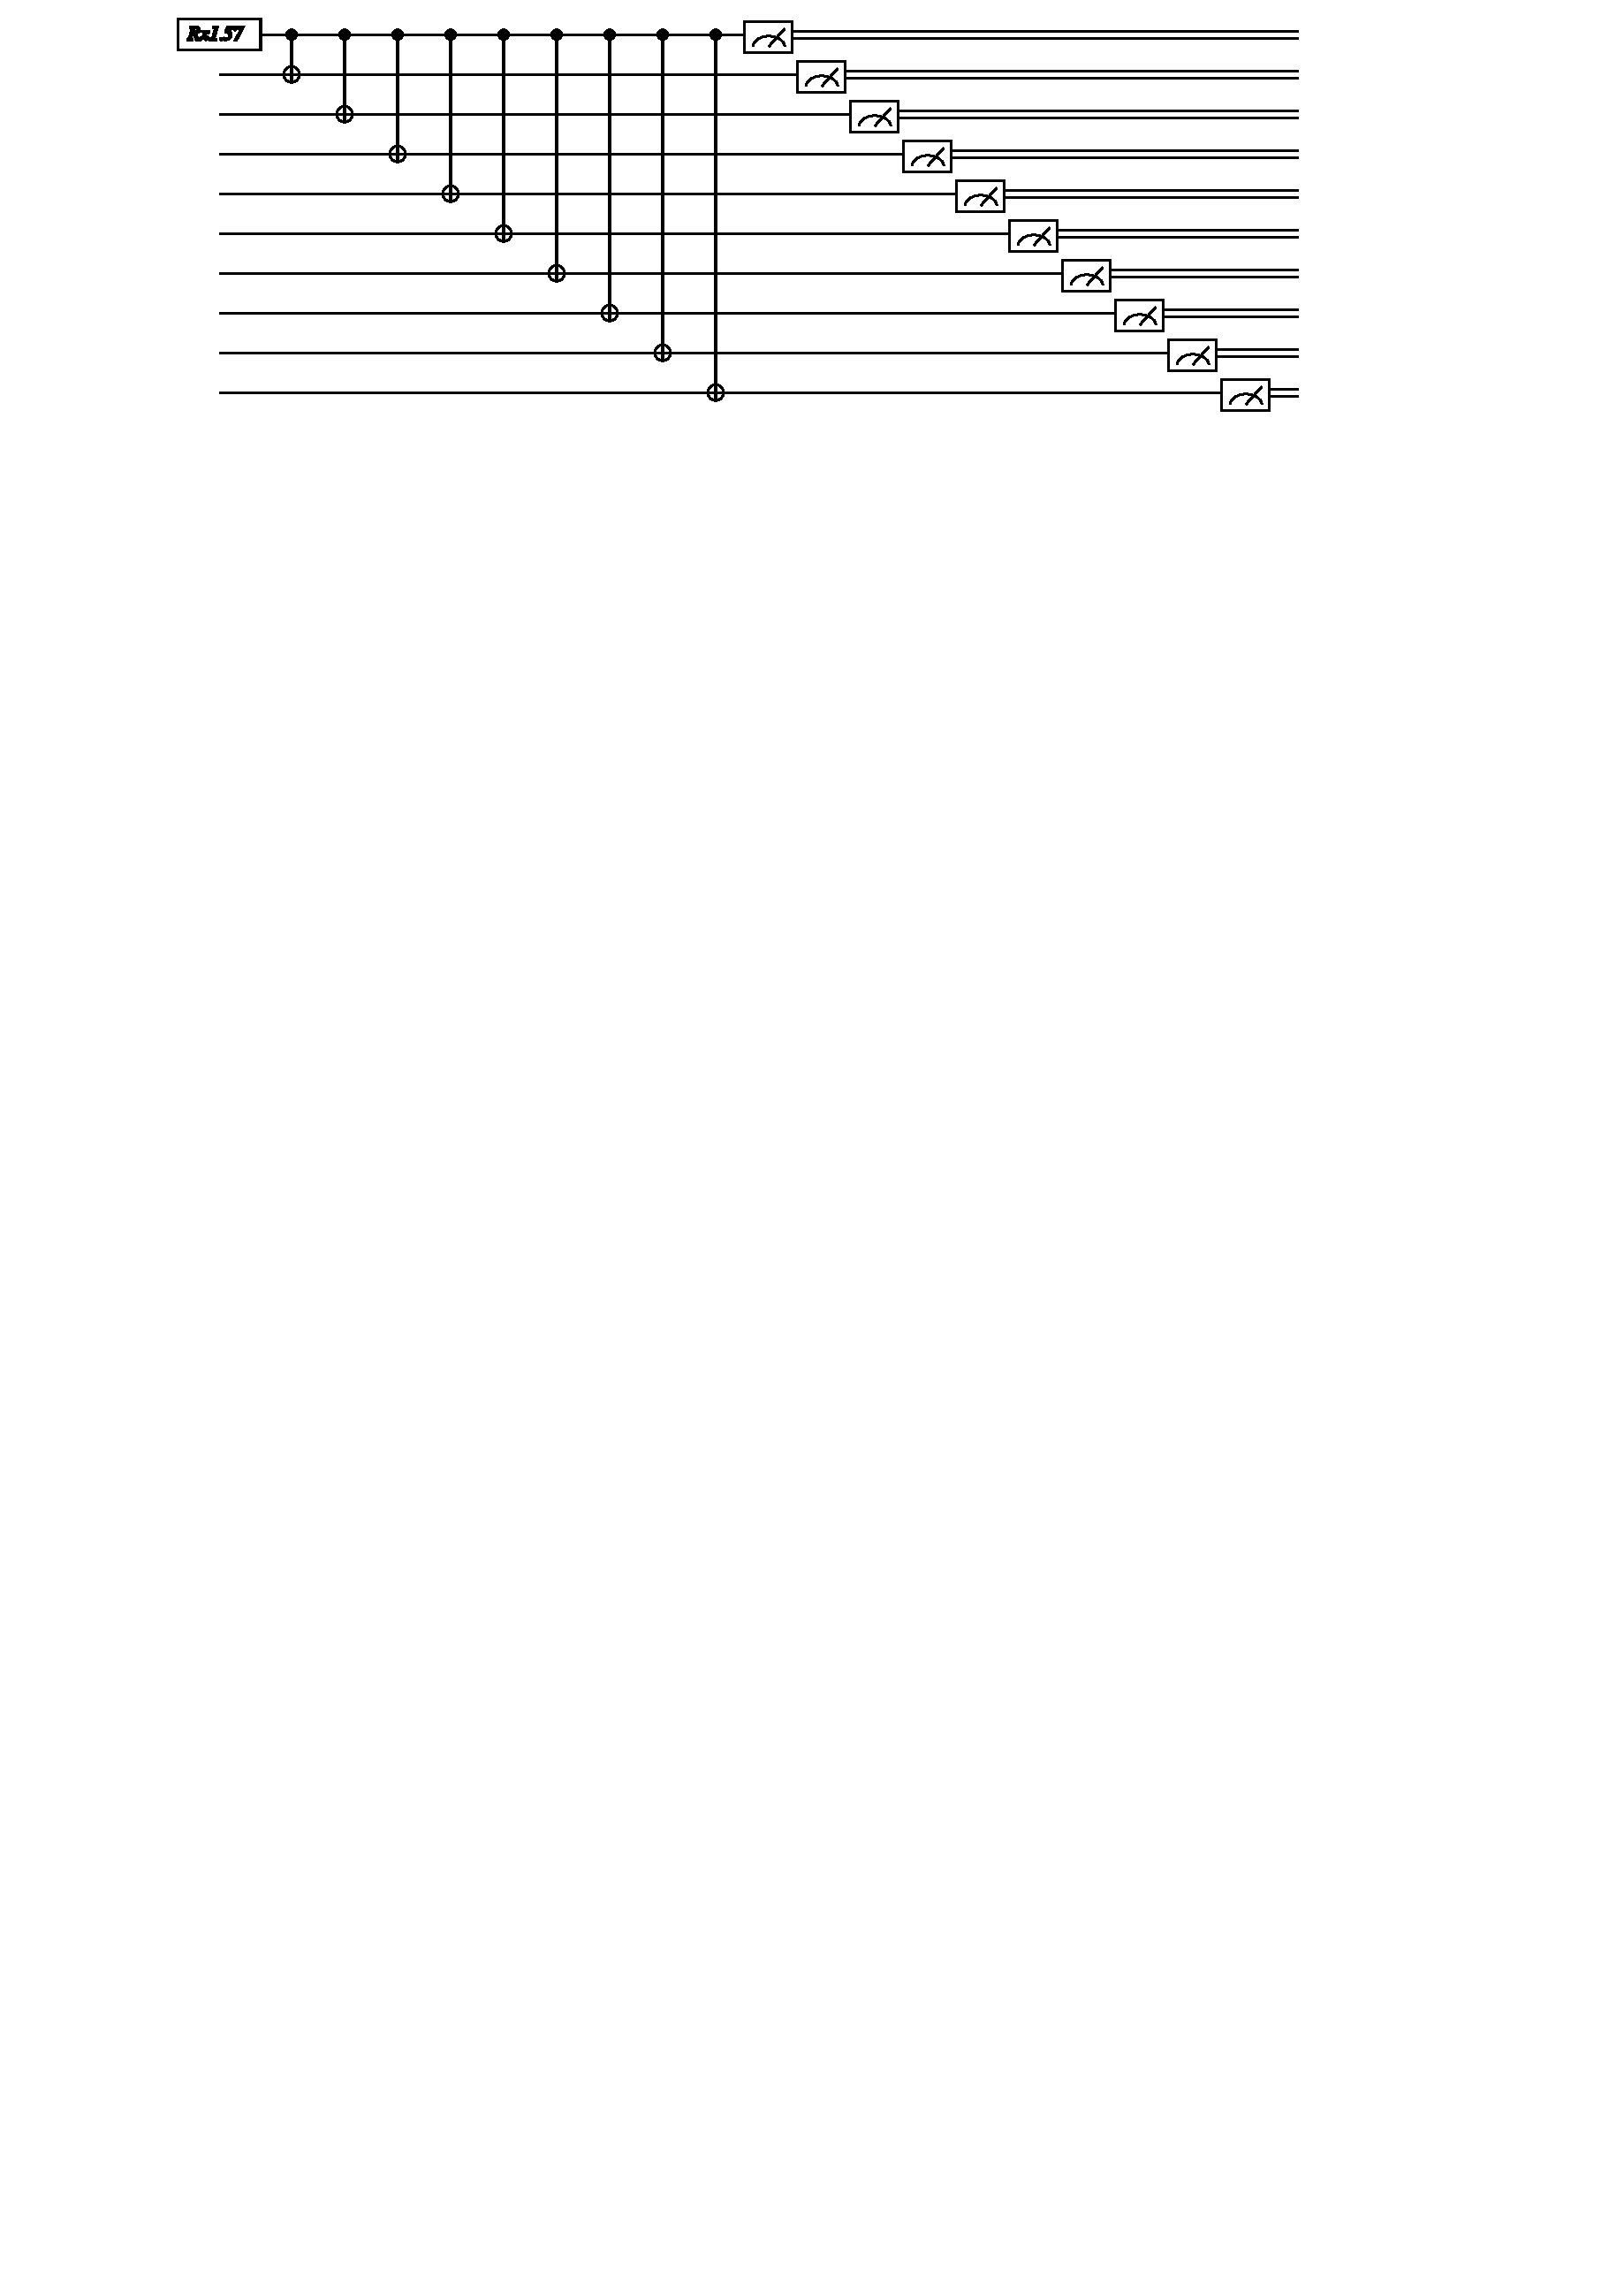
\includegraphics[width=15cm]{circuit1}
\caption{The initial state of the circuit}
\end{figure}
\begin{figure}[ht]
\centering
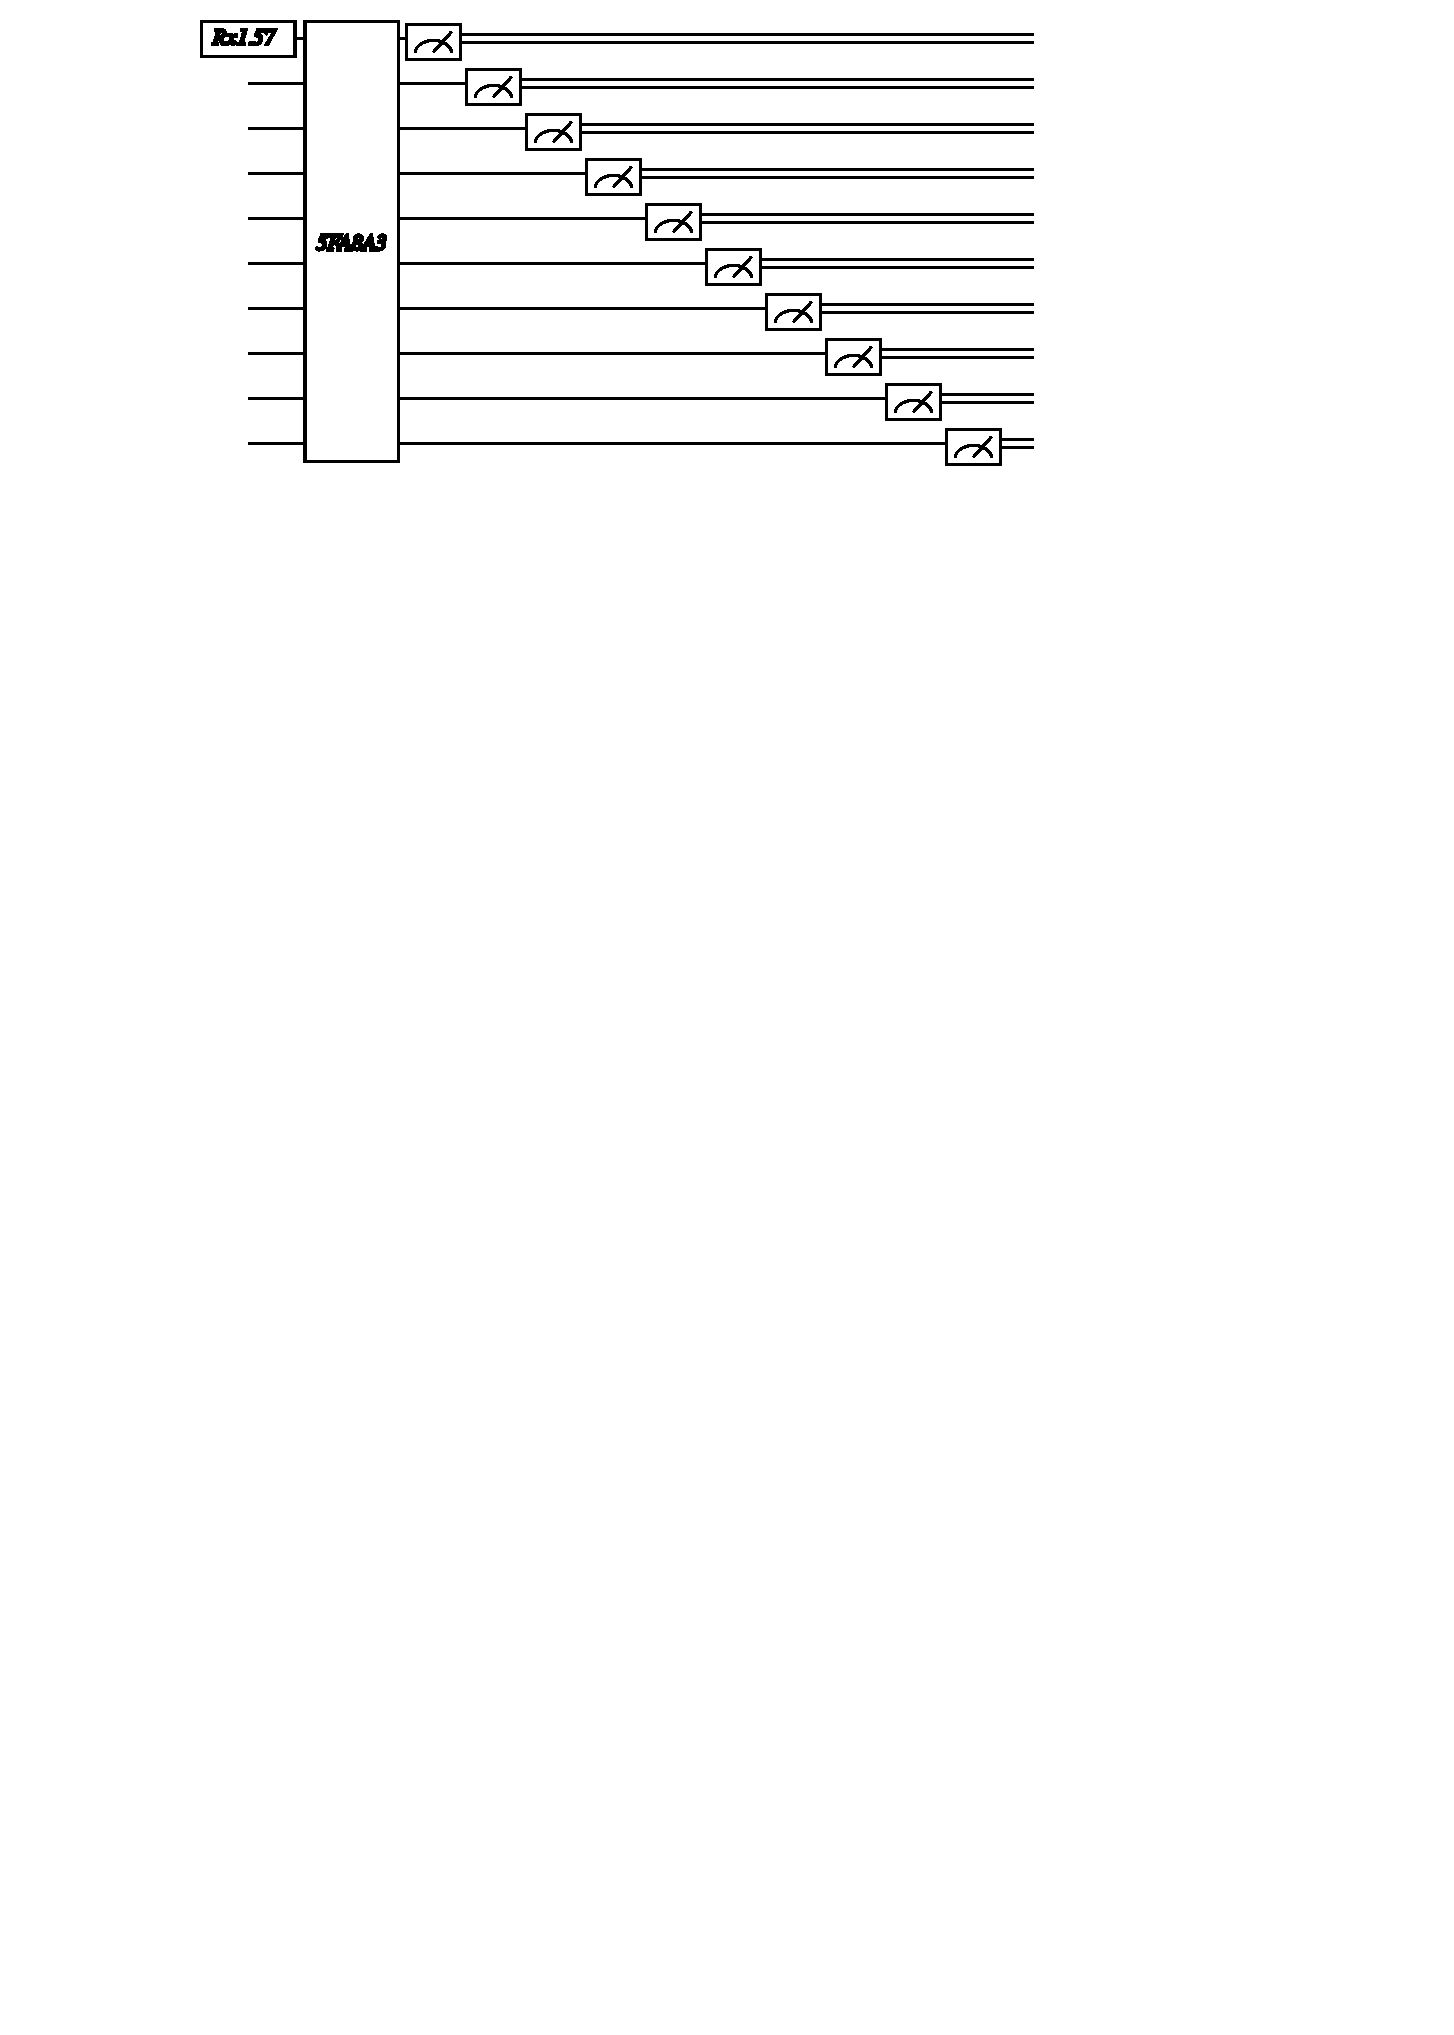
\includegraphics[width=10cm]{circuit2}
\caption{The circuit after being optimised}
\end{figure}

%\newpage
\section{Built-in Samples}
LIQ$Ui\ket{}$ contains a number of built-in samples for some of the specific quantum algorithms, including Shor’s algorithm, quantum teleportation, quantum error correction, quantum linear algebra, quantum associated memory and the simulation of the ground state energy of a molecule \cite{liquid-manual}. These executable samples gives users a glimpse of what LIQ$Ui\ket{}$ can do and application areas that it has been applied to. This section focuses on three built-in examples which are relevant to the concepts and applications explained in this report, including entanglement, Shor’s algorithm and quantum associative memory (utilising Grover’s algorithm) (See Appendix C for the list of all built-in samples).

\subsection{Entanglement}
This entanglement function produces detailed statistics the duration the simulator takes to perform various operations. It can be called with liquid \texttt{\_\_Entangle1(n)}, where $n$ is a number of qubits to be entangled (typically 10 to 22). The sample result is as the following:
\begin{verbatim}
0:0000.0/=============== Logging to: Liquid.log opened ================
0:0000.0/ Secs/Op  S/Qubit  Mem(GB) Operation
0:0000.0/ -------  -------  ------- ---------
0:0000.0/   0.035    0.035    0.019 Created single state vector
0:0000.0/   0.039    0.039    0.019 Did Hadamard
0:0000.0/   0.004    0.004    0.019   Did CNOT:  1
0:0000.0/   0.009    0.005    0.019   Did CNOT:  2
0:0000.0/   0.019    0.006    0.020   Did CNOT:  3
0:0000.0/   0.026    0.007    0.020   Did CNOT:  4
0:0000.0/   0.038    0.008    0.020   Did CNOT:  5
0:0000.0/   0.047    0.008    0.020   Did CNOT:  6
0:0000.0/   0.054    0.008    0.020   Did CNOT:  7
0:0000.0/   0.061    0.008    0.020   Did CNOT:  8
0:0000.0/   0.068    0.008    0.020   Did CNOT:  9
0:0000.0/   0.013    0.001    0.020 Did Measure
0:0000.0/=============== Logging to: Liquid.log closed ================
\end{verbatim}
Apart from above example, LIQ$Ui\ket{}$ also provides another two functions which perform quantum entanglement on qubits, namely \texttt{\_\_Entangle2} and \texttt{\_\_Entangles}. The \texttt{\_\_Entangle2} function operates in the same way with \texttt{\_\_Entangle1}. However, it also produces diagrams illustrating the circuits in the form of \texttt{htm} and \texttt{tex} files. The \texttt{\_\_Entangles} function runs a hundred entanglement tests on 16 qubits. At the end of the process, half of the qubits should be in state 1 and another half should be in the opposite state.

\subsection{Shor's Algorithm}
Shor's polynomial-time prime factorisation algorithm is one of the sophisticated built-in tests among other samples. The command \texttt{liquid \_\_Shor(n,true)} can be used to run the algorithm. The command takes two parameters. The first is the integer to be factored and the second is the option whether to optimise (by combining) the quantum circuit. The following is the result of prime factorisation using Shor's algorithm with 21 as an input:
\begin{verbatim}
0:0000.0/=============== Logging to: Liquid.log opened ================
0:0000.0/      21 = N = Number to factor
0:0000.0/       2 = a = coPrime of N
0:0000.0/       5 = n = number of bits for N
0:0000.0/      32 = 2^n
0:0000.0/      13 = total qubits
0:0000.0/      22 = starting memory (MB)
0:0000.0/  96.00% = prob of random result (983/1024)
0:0000.0/  43.07% = prob of Shor (worst case)
0:0000.0/         - Compiling circuit
0:0000.0/0.001330 = mins for compile
0:0000.0/   13890 = cnt of gates
0:0000.0/    3873 = cache hits
0:0000.0/     121 = cache misses
0:0000.0/      22 = compiled memory (MB)
0:0000.0/         - Wrapping circuit pieces
0:0000.1/            8 = wires have possibles: 66 (prv= 0GB did= 0 big= 0)
0:0000.1/            9 = wires have possibles: 57 (prv= 0GB did= 9 big= 4)
0:0000.1/           10 = wires have possibles: 52 (prv= 0GB did= 14 big= 39)
0:0000.1/           11 = wires have possibles: 51 (prv= 0GB did= 15 big= 81)
0:0000.2/           12 = wires have possibles: 48 (prv= 0GB did= 18 big= 124)
0:0000.2/           13 = wires have possibles: 47 (prv= 0GB did= 19 big= 166)
0:0000.2/      14 = Ran out of wires
0:0000.2/           MM: g:    19 b:   212  12=1 11=3 10=1 9=5 8=9
0:0000.2/0.140439 = mins for growing gates
0:0000.2/     470 = cnt of gates
0:0000.2/      52 = grown memory (MB)
0:0000.2/        Bit:   9 [MB:   49 m=1]
0:0000.3/        Bit:   8 [MB:   50 m=0]
0:0000.4/        Bit:   7 [MB:   49 m=1]
0:0000.6/        Bit:   6 [MB:   50 m=0]
0:0000.6/... compiling MB=      47 cache(15806,126) GC:8519
0:0000.8/        Bit:   5 [MB:   52 m=1]
0:0001.1/        Bit:   4 [MB:   52 m=0]
0:0001.2/        Bit:   3 [MB:   52 m=1]
0:0001.2/... compiling MB=      49 cache(27741,126) GC:6400
0:0001.4/        Bit:   2 [MB:   51 m=0]
0:0001.6/        Bit:   1 [MB:   53 m=1]
0:0001.8/        Bit:   0 [MB:   55 m=0]
0:0001.8/0.046182 = mins for running
0:0001.8/ 107.464 = Total Elapsed time (seconds)
0:0001.8/      13 = Max Entangled
0:0001.8/       0 = Gates Permuted
0:0001.8/     371 = State Permuted
0:0001.8/     128 = None  Permuted
0:0001.8/     341 = m = quantum result
0:0001.8/0.333008 = c = 341/1024 =~ 1/3
0:0001.8/        Odd denominator, expanding
0:0001.8/       3 = 6/2 = exponent
0:0001.8/       9 = 2^3 + 1 mod 21
0:0001.8/       7 = 2^3 - 1 mod 21
0:0001.8/       7 = factor = max(3,7)
0:0001.8/CSV N a m den f1 f2 good,21,2,341,6,7,3,1
0:0001.8/GOT:   21=   7x   3 co=    2 n,q=21,13 mins=1.79 SUCCESS!!
0:0001.8/=============== Logging to: Liquid.log closed ================
\end{verbatim}
According to the result, the quantum circuit had 13,890 gates that were reduced to 470 grown gates. The execution time is approximately 107 seconds on a Windows virtual machine with only 4 GB of RAM. However, the algorithm run successfully with the result $21 = 7\times3$.

\subsection{Quantum Associative Memory}
This built-in sample is the quantum associative memory algorithm developed by Dan Ventura and Tony Martinez \cite{qam}. The algorithm applies the theory of quantum physics in creating a quantum associative memory with an exponentially expanded capacity in the number of neurons. The first set of output is a number of key\/value pairs:
\begin{verbatim}
0:0000.0/Writing: QuAM1.htm (split=10.00% scale=70.00%)
0:0000.3/======= DUMPSTATE: Loaded patterns
0:0000.3/0x0a:  6.3% (0x001400)
0:0000.3/0x1a:  6.3% (0x003400)
0:0000.3/0x24:  6.3% (0x004800)
0:0000.3/0x3d:  6.3% (0x007a00)
0:0000.3/0x4b:  6.3% (0x009600)
0:0000.3/0x5e:  6.3% (0x00bc00)
0:0000.3/0x64:  6.3% (0x00c800)
0:0000.3/0x75:  6.3% (0x00ea00)
0:0000.3/0x8c:  6.3% (0x011800)
0:0000.3/0x9d:  6.3% (0x013a00)
0:0000.3/0xa6:  6.3% (0x014c00)
0:0000.3/0xb9:  6.3% (0x017200)
0:0000.3/0xcf:  6.3% (0x019e00)
0:0000.3/0xdd:  6.3% (0x01ba00)
0:0000.3/0xeb:  6.3% (0x01d600)
0:0000.3/0xf9:  6.3% (0x01f200)
\end{verbatim}
It is obvious that the circuit stored all the elements with equal probability. The next set of result demonstrates how the system used Grover's search algorithm to search for the element with key 6:
\begin{verbatim}
0:0000.3/Writing: QuAM2.htm (split=33.33% scale=70.00%)
0:0000.5/    Grover[ 0]: 0x64:  7.7% (0x00c800)
0:0000.5/    Grover[ 1]: 0x64: 12.4% (0x00c800)
0:0000.5/    Grover[ 2]: 0x64: 16.9% (0x00c800)
0:0000.5/    Grover[ 3]: 0x64: 19.2% (0x00c800)
0:0000.5/    Grover[ 4]: 0x64: 18.2% (0x00c800)
0:0000.5/    Grover[ 5]: 0x64: 14.5% (0x00c800)
0:0000.5/    Grover[ 6]: 0x64:  9.6% (0x00c800)
0:0000.5/    Grover[ 7]: 0x64:  5.5% (0x00c800)
0:0000.5/    Grover[ 8]: 0x64:  2.9% (0x00c800)
0:0000.5/    Grover[ 9]: 0x1a:  3.7% (0x003400)
0:0000.5/    Grover[10]: 0x1a:  3.8% (0x003400)
0:0000.5/    Grover[11]: 0x64:  3.2% (0x00c800)
0:0000.5/    Grover[12]: 0x64:  6.0% (0x00c800)
0:0000.5/    Grover[13]: 0x64: 10.3% (0x00c800)
0:0000.5/    Grover[14]: 0x64: 15.1% (0x00c800)
0:0000.5/    Grover[15]: 0x64: 18.6% (0x00c800)
0:0000.5/    Grover[16]: 0x64: 19.1% (0x00c800)

0:0000.5/======= DUMPSTATE: Searched for key: 6
0:0000.5/0x64: 19.1% (0x00c800)
0:0000.5/0x0a:  3.1% (0x001400)
0:0000.5/0x1a:  3.1% (0x003400)
0:0000.5/0x24:  3.1% (0x004800)
0:0000.5/0x3d:  3.1% (0x007a00)
0:0000.5/0x4b:  3.1% (0x009600)
0:0000.5/0x5e:  3.1% (0x00bc00)
0:0000.5/0x75:  3.1% (0x00ea00)
0:0000.5/0x8c:  3.1% (0x011800)
0:0000.5/0x9d:  3.1% (0x013a00)
0:0000.5/0xa6:  3.1% (0x014c00)
0:0000.5/0xb9:  3.1% (0x017200)
0:0000.5/0xcf:  3.1% (0x019e00)
0:0000.5/0xdd:  3.1% (0x01ba00)
0:0000.5/0xeb:  3.1% (0x01d600)
0:0000.5/0xf9:  3.1% (0x01f200)
0:0000.5/0x60:  1.7% (0x00c000)
0:0000.5/0x61:  1.7% (0x00c200)
0:0000.5/0x62:  1.7% (0x00c400)
0:0000.5/0x63:  1.7% (0x00c600)
\end{verbatim}
The result shows how Grover's algorithm performed the search through the optimal probability of finding the targeted key/value pair.

%\begingroup
%\renewcommand{\cleardoublepage}{}
%\renewcommand{\clearpage}{}
%\chapter{Evaluation}
%\endgroup

\chapter{Evaluation}

\noindent Practical quantum computing requires a toolchain extending from the level of abstract algorithm down to physical particles \cite{acm}. It is evident that experimenting quantum computing on a real quantum computer falls beyond the scope of this research report. This is the reason why LIQ$Ui\ket{}$ has been selected as a software architecture for quantum computing experiment since it allows users to express a quantum algorithm written in a high-level programming language (F\# in this case) into the low-level machine-readable instructions for a quantum computer \cite{liquid-overview}. \\\\
Ideally, a programming language to be translated into the machine instructions for a quantum device ought to allow developers to implement quantum algorithms in a human-comprehensible way \cite{acm}. This means the language should support a level of abstraction that is close to the way one naturally thinks about how the algorithm should be implemented. For example, if the quantum algorithm is primarily expressed by a computationally mathematical formula, the programming language used to implement that kind of algorithm should support such expression. Fortunately, F\# is a multi-paradigm programming language with a sufficient level of flexibility to fulfill that requirement. \\\\
By using LIQ$Ui\ket{}$ as a quantum computing simulator, users are able to simulate various quantum algorithms along with other quantum operations, such as expressing quantum circuits using a high-level functional language (F\#), extracting circuit data structure for circuit optimisation, gate replacement, quantum error correction, circuit rendering and export \cite{liquid-overview}. In essence, LIQ$Ui\ket{}$ allows users to experiment and understand how quantum computing can be applied to various real-world applications.

%\begingroup
%\renewcommand{\cleardoublepage}{}
%\renewcommand{\clearpage}{}
%\chapter{Reflection}
%\endgroup

\chapter{Reflection}

\noindent The computational power of quantum computing is based on the laws of quantum physics and various quantum phenomena, such as quantum entanglement,  quantum parallelism or quantum interference \cite{acm}. Those events are radically different from what can be encountered in classical computing. Consequently, in order to comprehend these attributes and designs algorithms that outperform the well-known classical counterparts, it is mandatory to understand the fundamental principles of quantum computing as well as why some certain problems cannot be solved by a conventional digital computer. \\\\
Apart from the comprehension of the principles which quantum mechanic is based on, it is also necessary to understand the programming aspect of how to express a quantum algorithm in the form of a high-level program which will be translated into a set of instructions for a quantum computer. Even though LIQ$Ui\ket{}$ already enables easy programming and compilation for the simulation of quantum algorithms and circuits, having knowledge of the functional programming paradigm also results in increased ease in the algorithm implementation process since the simulator adopts a high-level functional programming language (F\#) as its host language. \\\\
Most of the modern quantum programming languages may be taxonomically classified into the imperative paradigm, the functional paradigm and others \cite{qc-languages}. However, many of recent quantum programming developments have focused on utilising functional quantum programming languages instead of imperative quantum programming languages due to its succinctness \cite{functional}, which allows developers to express algorithms more clearly. Hence, it is valuable to understand the concept of functional programming as an alternative way of thinking and expressing algorithms for either classical or quantum computation, apart from programming in the imperative style which most of the developers have been accustomed.

\bibliography{refs} % this causes the references to be listed
\bibliographystyle{apacite} % bibliography style
\nocite{liquid-manual,circuit-tut}

%% Appendices start here
\appendix

\titleformat{\chapter}{\normalfont\huge\bf}{\chaptertitlename \ \thechapter\ \ \ --}{20pt}{\huge\bf} 

\chapter{Quantum Fourier Transform}

According to the definition of the quantum Fourier transform (QFT), it is the discrete Fourier transform (DFT) applied to the amplitudes of a quantum state that performs a linear transformation on qubits \cite{washington}. The DFT is a version of Fourier transform that performs a transformation on a discrete number of frequencies and discrete-time signal. The DFT of a vector can be defined as:
$$\tilde{f}(k)=\frac{1}{\sqrt[]{N}}\sum_{j=0}^{N-1}e^{2\pi i(\frac{jk}{N})}f(j)$$ \\
The QFT is considered the same transformation as the DFT. However, since the transformation occurs on the qubit states, a unitary operator $F$ on $n$ qubits $(N=2^n)$ must be defined as:
$$F\ket{j}=\frac{1}{\sqrt[]{2^n}}\sum_{j=0}^{2^n-1}e^{2\pi i(\frac{jk}{2^n})}\ket{k}$$\\
For example, the transformation coefficient of a two-qubit quantum register can be expressed as the following:
$$\ket{j}\rightarrow\frac{1}{2}(\ket{00}+e^{2\pi i\frac{j}{4}}\ket{01}+e^{2\pi i\frac{j2}{4}}\ket{10}+e^{2\pi i\frac{j3}{4}}\ket{11})$$ \\
Thus, the QFT of $\ket{j}$ can be represented as:
$$\ket{00}\rightarrow\frac{1}{2}(\ket{00}+\ket{01}+\ket{10}+\ket{11}$$
$$\ket{01}\rightarrow\frac{1}{2}(\ket{00}+\omega\ket{01}+\omega^2\ket{10}+\omega^3\ket{11}$$
$$\ket{10}\rightarrow\frac{1}{2}(\ket{00}+\omega^2\ket{01}+\omega^4\ket{10}+\omega^6\ket{11}$$
$$\ket{11}\rightarrow\frac{1}{2}(\ket{00}+\omega^3\ket{01}+\omega^6\ket{10}+\omega^9\ket{11}$$ \\
Essentially, the QFT maps the standard basis state $(\ket{j})$ to the Fourier basis stage. The transformation is also unitary, which allows high efficiency when performing on a quantum computer.

\chapter{LIQ$Ui\ket{}$ Experiment}

\section{Entanglement Source Code}
\begin{verbatim}
#if INTERACTIVE
#r @"..\bin\Liquid1.dll"                 
#else
namespace Microsoft.Research.Liquid // Namespace
#endif

open System                         // Support libraries
open Microsoft.Research.Liquid      // Liquid libraries
open Util                           // General utilites
open Operations                     // Basic gates and operations

// Rotates a qubit around any arbitrary angle in the X axis 
let rotationX (theta:float) (qs:Qubits) =
    let gate (theta:float) =
        let name = "Rx" + theta.ToString("F2")
        new Gate(
            Name = name,
            Help = sprintf "Rotate in X by: %f" theta,
            Mat = (
                let phi = theta / 2.0
                let c = Math.Cos phi
                let s = Math.Sin phi
                CSMat(2,[0,0,c,0.;0,1,-s,0.;1,0,s,0.;1,1,c,0.])),
            Draw    = "\\gate{" + name + "}"
            )
    (gate theta).Run qs
    
// Quantum funtion
let quantumFunction (qubits:Qubits) =
    rotationX (Math.PI/2.0) qubits
    for qubit in qubits.Tail do 
        CNOT [qubits.Head; qubit]
    M >< qubits // Measures all the qubits




[<LQD>]
let Liquid(n:int) =
    let stats = Array.create 2 0
    let ket = Ket(n)
    let circuit = Circuit.Compile quantumFunction ket.Qubits
    show "Circuit 1:"
    circuit.Dump()
    circuit.RenderHT("Circuit1")
    let circuit = circuit.GrowGates(ket)
    show "Circuit 2:"
    circuit.Dump()
    circuit.RenderHT("Circuit2")
    for i in 0..999 do
        let qubits = ket.Reset(n) 
        circuit.Run qubits
        let value = qubits.Head.Bit.v
        stats.[value] <- stats.[value] + 1
    show "Measured: 0 = %d 1 = %d" stats.[0] stats.[1]
\end{verbatim}

\section{LIQ$Ui\ket{}$ Log File}
\begin{verbatim}
0:0000.0/=============== Logging to: Liquid.log opened ================
0:0000.1/Circuit 1:
0:0000.1/SEQ
0:0000.1/  APPLY
0:0000.1/    GATE Rx1.57 is a Rotate in X by: 1.570796 (Normal) 
0:0000.1/      0.7071 -0.7071 
0:0000.1/      0.7071 0.7071 
0:0000.1/    WIRE(Id:0)
0:0000.1/    WIRE(Id:1)
0:0000.1/    WIRE(Id:2)
0:0000.1/    WIRE(Id:3)
0:0000.1/    WIRE(Id:4)
0:0000.1/    WIRE(Id:5)
0:0000.1/    WIRE(Id:6)
0:0000.1/    WIRE(Id:7)
0:0000.1/    WIRE(Id:8)
0:0000.1/    WIRE(Id:9)
0:0000.1/  APPLY
0:0000.1/    GATE CNOT is a Controlled NOT (Normal) 
0:0000.1/      1 0 0 0 
0:0000.1/      0 1 0 0 
0:0000.1/      0 0 0 1 
0:0000.1/      0 0 1 0 
0:0000.1/    WIRE(Id:0)
0:0000.1/    WIRE(Id:1)
0:0000.1/  APPLY
0:0000.1/    GATE CNOT is a Controlled NOT (Normal) 
0:0000.1/      1 0 0 0 
0:0000.1/      0 1 0 0 
0:0000.1/      0 0 0 1 
0:0000.1/      0 0 1 0 
0:0000.1/    WIRE(Id:0)
0:0000.1/    WIRE(Id:2)
\end{verbatim}
\vdots
\begin{verbatim}
0:0000.1/Circuit 2:
0:0000.1/SEQ
0:0000.1/  APPLY
0:0000.1/    GATE Rx1.57 is a Rotate in X by: 1.570796 (Normal) 
0:0000.1/      0.7071 -0.7071 
0:0000.1/      0.7071 0.7071 
0:0000.1/    WIRE(Id:0)
0:0000.1/    WIRE(Id:1)
0:0000.1/    WIRE(Id:2)
0:0000.1/    WIRE(Id:3)
0:0000.1/    WIRE(Id:4)
0:0000.1/    WIRE(Id:5)
0:0000.1/    WIRE(Id:6)
0:0000.1/    WIRE(Id:7)
0:0000.1/    WIRE(Id:8)
0:0000.1/    WIRE(Id:9)
0:0000.1/  APPLY
0:0000.1/    GATE 5FA8A3 is a 5FA8A3 (Normal) 
0:0000.1/       0  0 1
0:0000.1/       1  1 1
0:0000.1/       2  2 1
0:0000.1/       3  3 1
0:0000.1/       4  4 1
0:0000.1/       5  5 1
0:0000.1/       6  6 1
0:0000.1/       7  7 1
\end{verbatim}
\vdots
\begin{verbatim}
0:0000.1/Measured: 0 = 484 1 = 516
0:0000.1/=============== Logging to: Liquid.log closed ================
\end{verbatim}

\chapter{Built-in Samples}

\begin{verbatim}
===================================================================================
=   The Language-Integrated Quantum Operations (LIQUi|>) Simulator                =
=   Copyright (c) 2015,2016 Microsoft Corporation                                 =
=   If you use LIQUi|> in your research, please follow the guidelines at          =
=   https://github.com/msr-quarc/Liquid for citing LIQUi|> in your publications.  =
===================================================================================

TESTS (all start with two underscores):
__Big()             Try to run large entanglement tests (16 through 33 qubits)
__Chem(m)           Solve Ground State for molecule m (e.g., H2O)
__ChemFull(...)     See QChem docs for all the arguments
__Correct()         Use 15 qubits+random circs to test teleport
__Entangle1(cnt)    Run n qubit entanglement circuit (for timing purposes)
__Entangle2(cnt)    Entangle1 with compiled and optimized circuits
__Entangles()       Draw and run 100 instances of 16 qubit entanglement test
__EntEnt()          Entanglement entropy test
__EIGS()            Check eigevalues using ARPACK
__EPR()             Draw EPR circuit (.htm and .tex files)
__Ferro(false,true) Test ferro magnetic coupling with true=full, true=runonce
__JointCNOT()       Run CNOTs defined by Joint measurements
__Noise1(d,i,p)     d=# of idle gates, i=iters, p=probOfNoise
__NoiseAmp()        Amplitude damping (non-unitary) noise
__QECC()            Test teleport with errors and Steane7 code (gen drawing)
__QFTbench()        Benchmark QFT used in Shor (func,circ,optimized)
__QLSA()            Test of HHL linear equation solver
__QuAM()            Quantum Associative Memory
__QWalk(typ)        Walk tiny,tree,graph or RMat file with graph information
__Ramsey33()        Try to find a Ramsey(3,3) solution
__SG()              Test spin glass model
__Shor(N,true)      Factor N using Shor's algo false=direct true=optimized
__show("str")       Test routine to echo str and then exit
__Steane7()         Test basic error injection in Steane7 code
__Teleport()        Draw and run original, circuit and grown versions
__TSP(5)            Try to find a Traveling Salesman solution for 5 to 8 cities
\end{verbatim}

\end{document}